\usetikzlibrary{arrows.meta}
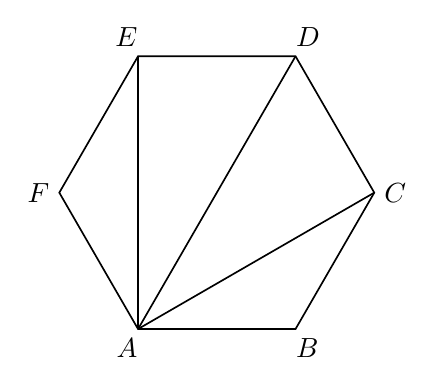
\begin{tikzpicture}[x=1cm,y=1cm,font=\normalsize]
% Q16 Jiangxi: regular hexagon side 2, A origin
\coordinate (A) at (0,0);
\coordinate (B) at (2,0);
\coordinate (C) at (3,1.7320508075688772);
\coordinate (D) at (2,3.4641016151377544);
\coordinate (E) at (0,3.4641016151377544);
\coordinate (F) at (-1,1.7320508075688772);
\draw[line width=.6pt] (A) -- (B) -- (C) -- (D) -- (E) -- (F) -- cycle;
\draw[line width=.6pt] (E) -- (A);
\draw[line width=.6pt] (D) -- (A);
\draw[line width=.6pt] (C) -- (A);
% labels outside vertices
\node[inner sep=0pt,font=\normalsize,below left] at (0,-0.12) {$A$};
\node[inner sep=0pt,font=\normalsize,below right] at (2,-0.12) {$B$};
\node[inner sep=0pt,font=\normalsize,right] at (3.12,1.7320508075688772) {$C$};
\node[inner sep=0pt,font=\normalsize,above right] at (2,3.58) {$D$};
\node[inner sep=0pt,font=\normalsize,above left] at (0,3.58) {$E$};
\node[inner sep=0pt,font=\normalsize,left] at (-1.12,1.7320508075688772) {$F$};
\end{tikzpicture}
